\documentclass{aastex62}
\begin{document}
\title{Homework 1 \\ G 254-34: Finding and Observation Charts}
\section{Introduction}
Location data obtained from http://simbad.u-strasbg.fr/simbad/sim-id?Ident=\%40408574\&Name=G\%20254-34\&submit=submit .

G 254-34 is a High proper-motion star located at right ascension 12 04 45.3706777541 and declination +75 20 57.322940366 in epoch J2000. 

\begin{center}
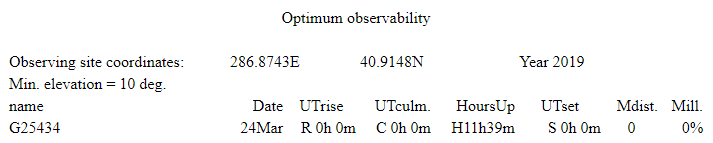
\includegraphics[scale=0.6]{optimum.PNG}
\end{center}


\section{Finding Chart}
\begin{center}
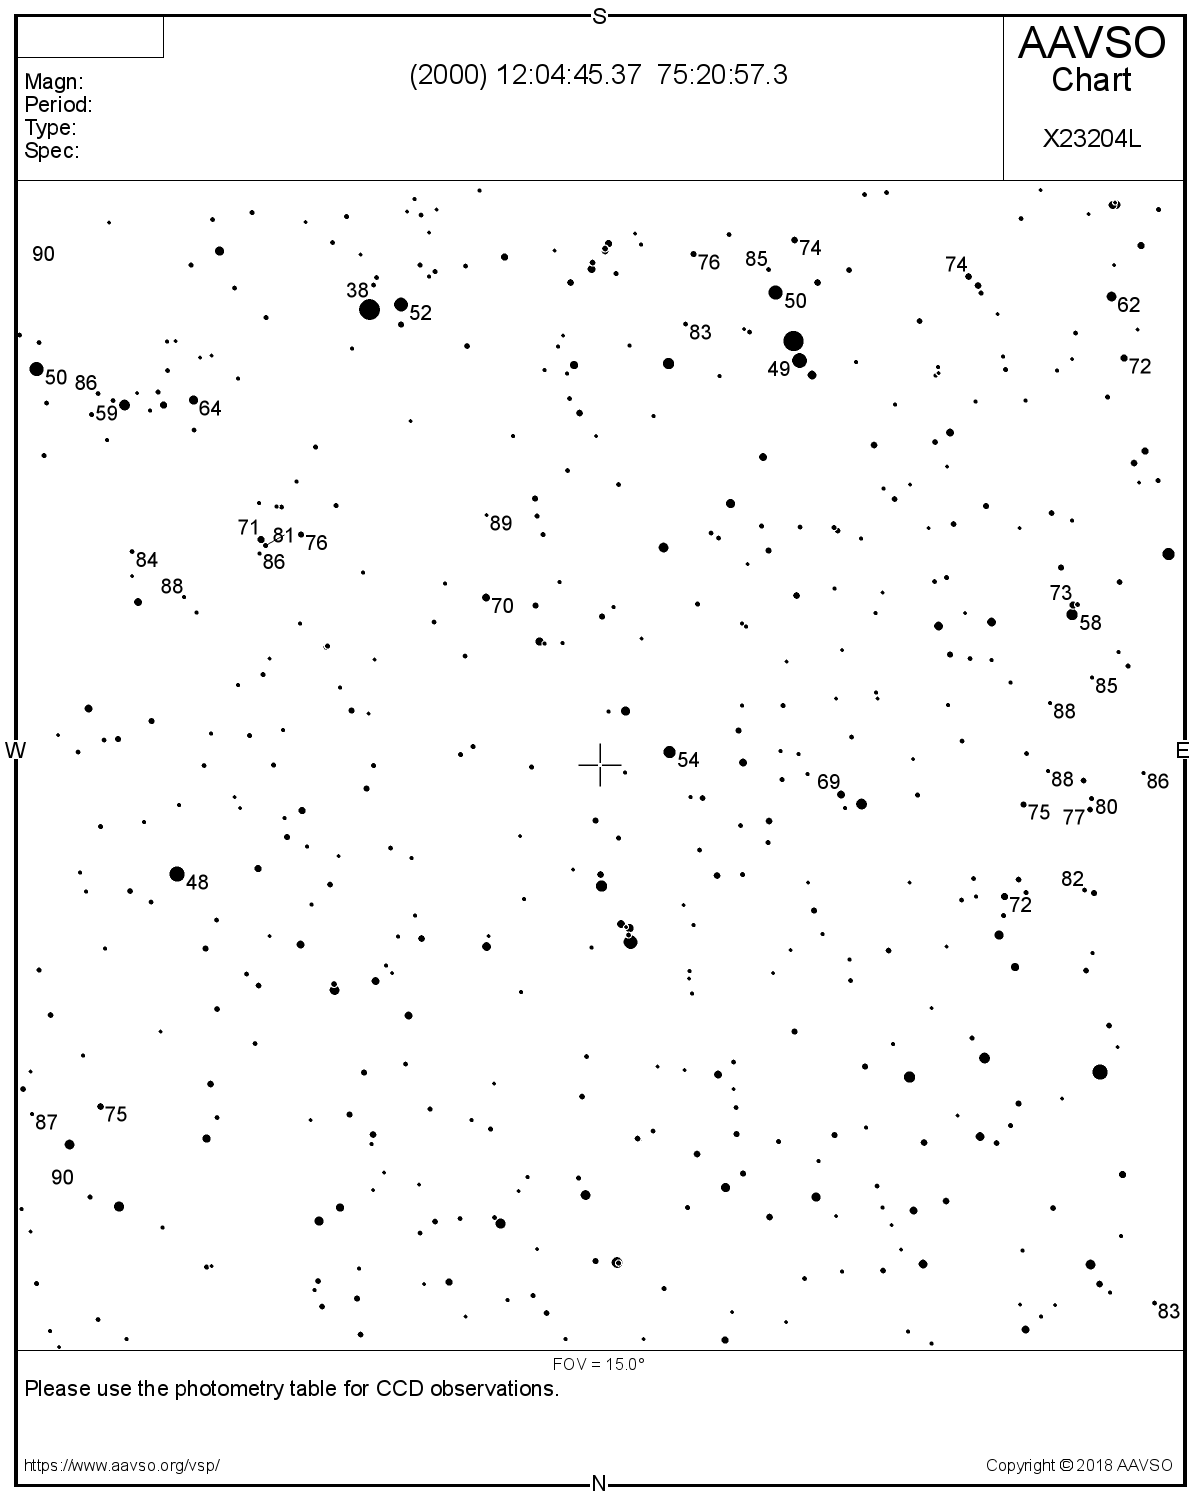
\includegraphics[scale=0.34]{Chart.png}
\end{center}

\newpage
\section{Altitude and Track}

\begin{figure}[ht!]

\gridline{\fig{staralt_pdf.pdf}{0.5\textwidth}{(a)}
          \fig{Ideal_staralt_pdf.pdf}{0.5\textwidth}{(b)}
          }
\gridline{\fig{startrack_pdf.pdf}{0.5\textwidth}{(c)}
          \fig{Ideal_startrack_pdf.pdf}{0.5\textwidth}{(d)}
          }
\caption{In (a) is the altitude of G 254-34 on the day of writing, (b) shows the altitude on the optimal observation day (March 24). The charts in (c) and (d) show the tracks on the day of writing and the optimal observation day, respectively. Dotted curves represent the Moon.}
\end{figure}

\newpage
\section{Monthly Observation}

\begin{figure}[ht!]
\plotone{starobs_pdf.pdf}
\caption{Altitude throughout the year. Note, the star does not go below 10 degrees altitude.}
\end{figure}

\end{document}